\documentclass[USenglish]{article}

\usepackage[utf8]{inputenc}
\usepackage[small]{dgruyter}
\usepackage{microtype}
\usepackage{graphicx}
%\graphicspath{ {./images/} }

\begin{document}

  \articletype{...}

  \author*[1]{...}
  \author[2]{...}
  \author[1]{...} 
  \runningauthor{...}
  \affil[1]{...}
  \affil[2]{...}
  \title{...}
  \runningtitle{...}
  \subtitle{...}
  \abstract{...}
  \keywords{...}
  \classification[PACS]{...}
  \communicated{...}
  \dedication{...}
  \received{...}
  \accepted{...}
  \journalname{...}
  \journalyear{...}
  \journalvolume{..}
  \journalissue{..}
  \startpage{1}
  \aop
  \DOI{...}

\maketitle


- we are assuming good-quality (even if not perfect) input data
- including full details of age and cohorts
- we will focus on countries with good quality data (though we believe that demographic accounts also useful for countries with poor data)


target audience: official statistics agencies in countries with good data

outline of paper
- introduction
  - demographic accounts have same origin as national accounts
  - have same advantages - eg common format, framework, accounting identities to infer missing quantities
  - but demography has better data!
    - motivating example: greenland 
    - why greenland?
        - because has published account - automated, API
        - much more detailed and integrated than most (because has Lexis triangles)
     - main advantage: standard format that can be used for many purposes, same format for forecasts, modelling, all different series, cross-country comparison, non-demographic variables [sex, region, place of birth categories  - but also income, education, occupation] - cite Richard Stone
    - although we consider more widely
- greenland data (or countries with population registers??)
  - raw data
  - processed data
- *published* account for greenland
  - very aggregated
  - national
  - subnational
- why it is useful (for greenland)
    - data corrections (note - will discuss further below)
    - understanding Greenland demographic system (eg movements to/from Denmark)
    - transparency eg in forecasting
    - make it easy for people to get data on demographic change, all in one place - and understand
    - better scenario analysis
 - dealing with inconsistencies
    - including 'corrections' in account (analogous to national account)
    - can use estimation methods to make it consistent
       - maybe give example using 'demest'?? (small example)
  - dissemination
     - stat bank system
     - ease of getting data
     - common conventions on what the data should look like (to go with common software)
     - how to disseminate uncertainty?
  - discussion: implications for other countries
    - can other countries emulate Greenland?
       - countries with good data
       - countries with bad data
    - why is it also useful in other countries
    - can countries without population registers emulate greenland
    - many agencies do accounting implicitly, adhoc
    denmark published from 1975-2004, then stopped ) :
    - accounts for holland, faroe islands
    
    
    - 
- 
- 

\section{What is a demographic account}


\section{Why are demographic accounts useful?}





\section{Focus of paper}

opening statement? why this paper?

greenland has registerbased, almost perfect data to model its population and publish detailed data, accessible by api in a popacc.

for countries with less detailed data a popaccount on local level can be estimated using bayes methods demonstrated with project greenlandaccount 

the methods can be compared with the greenlandic data  

no matter how a country's pop is estimated, the popacc can serve as a full repository for all demograhic meassures and forecasts. in most stat offices the info is gathered by many specialized employees, the popacc will bring this knowledge together




- arguments [and good showcases] for demographic accounts

larp: from the popaccount I now extract data that serve as input to mortality.org step 2, generates HMD data tables, step 3 run all code that uses this format. 

- to convince countries we have to show that they can be used

- Nico Kielman: does not need account because he gets the data anyway
- places like HMD very specific in their focus
- HFD is another project
- to do forecasts need more info
- need general way to have population accounts - then others would use them
- lots of interest in local level details
- demographic accounts are likely to be useful for local level


- iceland migration paper
   - Lars reproducing with Greenland data
   - internal migration could be included in account with satellite table
   - could add origin-destination to core regional table
   - fertility could be a satellite table with mother's age
- applications of regional accounts
   - population forecasts
   - regional analyses of mortality
   - 
- lots of interest in local demographic change
    - to understand need to have all components of change
    - need to present data in a form that people can download and look at themselves
    
- Lars wants to do non-black box forecasts for Greenland, including publishing the code on github
- it can be hard for people to get hold of data - hasn't improved since the 1990s

larp: the technical possibilities have exploded. api's in place for 5 years now. cannot remember this argument. 

- pxweb - accessible data - include this as a part of the wider package of a 'demographic account'

infrastructure
- data collection (popn registers in Greenland)
- reconciliation
- public dissemination

Nordic countries - can combine everything via personal ID

What about countries without population registers?
- a population count is a *model* of the population
- if a country does not have a population register but can estimate it, then they can still do an account; and reconcile via stat method
- need to be transparent but it best that can be produced
- we use National Accounts - even though they are badly imperfect
- in Copenhagen, demographic accounts where part of the demography mainstream

the Danish Population account on national level was published from 1975 to 2004 on paper. 

a lot of demographic accounting is implicit

- in nordic countries individual-level data is available - everyone concentrates on that

- don't need individual-level data for accounts

- demographic analyses are tied to aggregate-level analysis
- advantages of aggregate-level analysis
   - does not invade privacy, can be transparent
   - some processes, concepts are intrinsically aggregate - eg demographic

- account has to be designed to be meaningful for the society
- what variables are included etc
- dimensions will vary from place

- Why is Eurostat not interested in demographic accounts?
    - want to gather info at disaggregated level with Lexis triangles
    - Eurostat is doing something (UNIDEMO)
    - 

\section{Introduction} 
The Population Account for Greenland offers a set of coherent tables that allows calculations of all demographic measures at aggregated level.

A core table holds totals of demographic events that  explains annual change in the population size. The sum of birth surplus and net migration makes up the difference in annual population estimates, but will only be accurate in a world with perfect data. In all practical situations there need to be a hopefully small correction figure added, to make the account coherent. At the same time, analysis of corrections offers valuable information on possible data problems, Statistics Greenland should aim to improve.

The account can be broken down in categories like ‘place of birth’, sex and region and also from three variables ‘year of birth’, time and lexis-triangle, age can be calculated. 

This is a sufficiently detailed table to serve as a model of the Greenlandic population ready to be consumed for descriptive purposes or as baseline in projections.

At national level totals of net internal migration is per definition equal zero, but in regional forecasts movings between regions are essential in order to predict the size, sex and age distribution in the regions. Instead of adding dimensions on origin and destination to the core account, a satellite table focus on internal migrations.

The same goes for number of live born. They too are accessible in a satellite table with dimensions ‘sex of child’ and on mother: ‘place of birth’, ‘year of birth’, age, region and time.



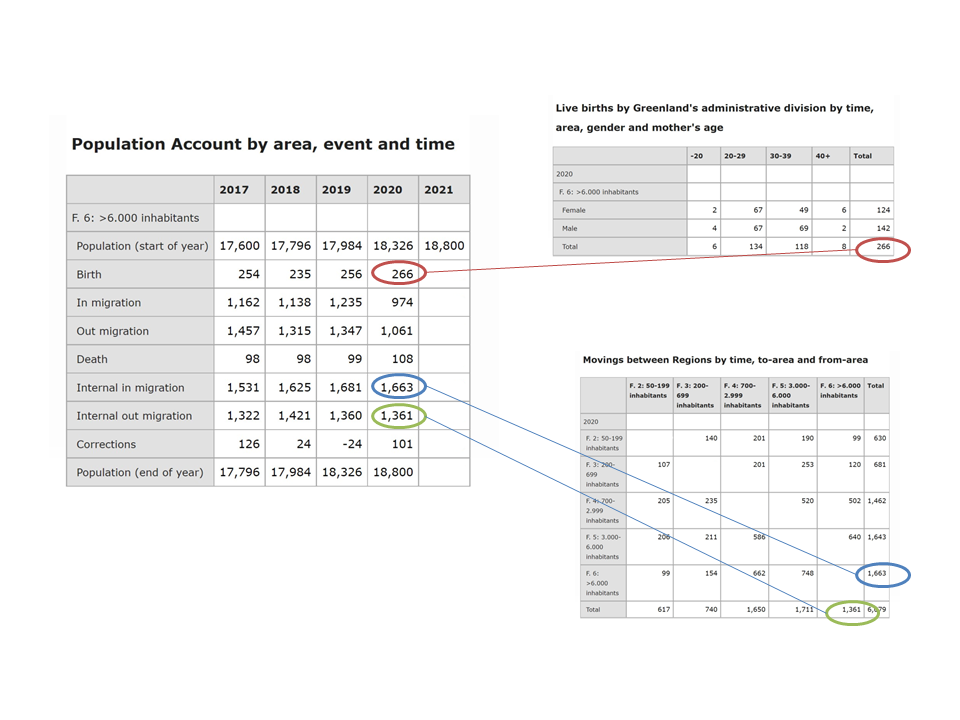
\includegraphics[scale=0.4]{images/PopulationAccountCoreSatellite}

category dimensions (sex, place of birth) can be filtered some with alternate classifications

other fixed category dimensions could be relevant: 

categories changing over time:
citizenship, education, income, marital status


\subsection{Dimensions in core table} 
The central dimension in the core table is called ‘event’ eventhough it also holds population estimate at start and end of year. Population at start of year plus the sum of net-events equals population at end of year/start of the following year.

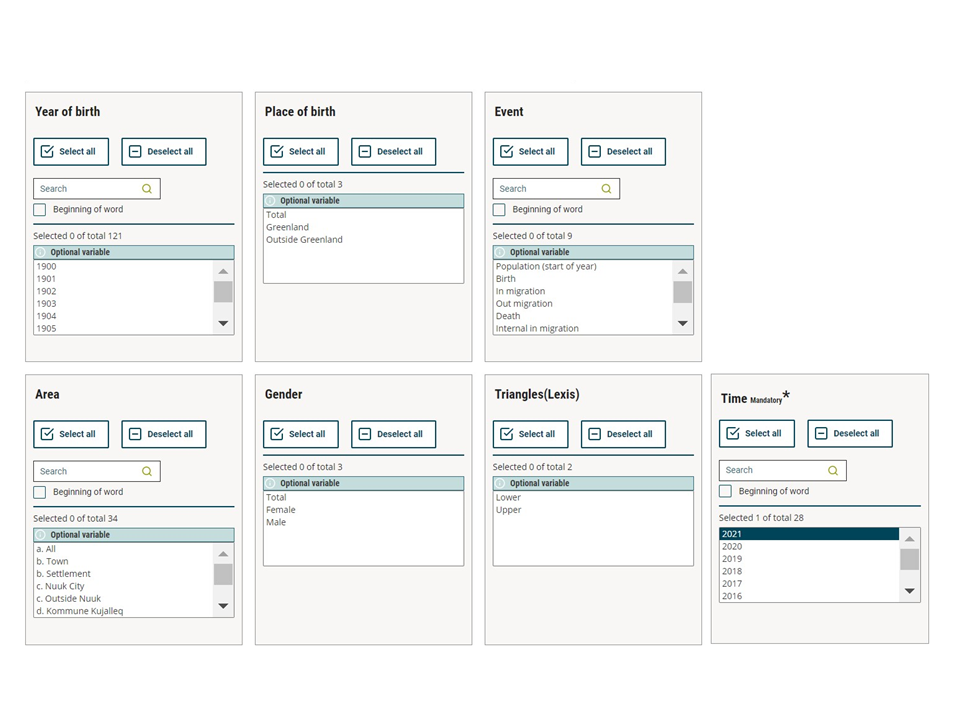
\includegraphics[scale=0.4]{images/PopulationAccountCore}
Filter dimensions are: area, ‘Place of Birth’ and gender, but the Greenlandic statistical system could provide altenate dimensions like ancestry, education, marital status, income


\subsection{Age at event} 

The Statbank Greenland, core table does not have an age dimension, instead age-at-event has to be calculated from ‘year of birth’ (cohort) and time (period) as time dimensions.

To allow calculation at time of event a ‘triangles(lexis)’-dimension is provided. This enables calculation of age, at time of event. The vertical parallelogram counts events that are defined by calendar year and year of birth (cohort) - accross 2 agespans. Knowing that events occured before or after a persons birthday in a calendar year, is needed to calculate persons age at event, but then is easily calculated:

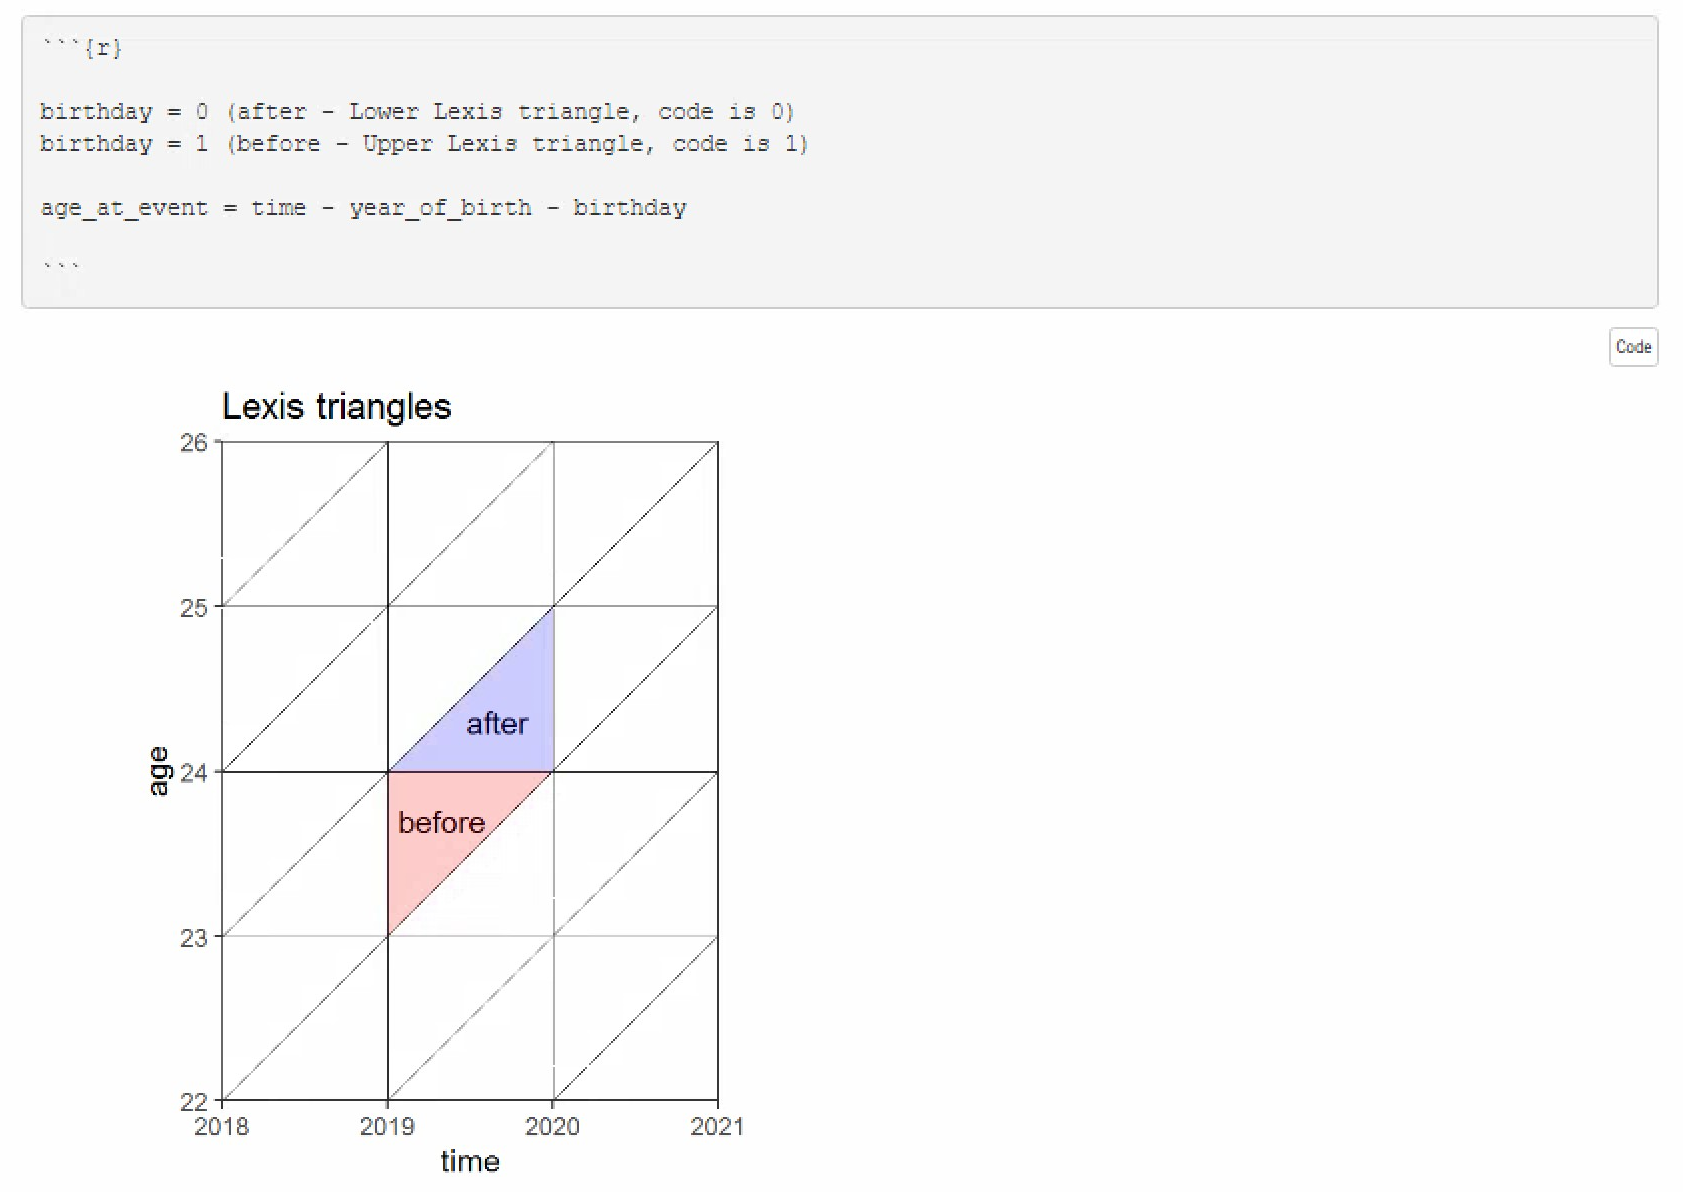
\includegraphics[scale=0.25]{images/PopulationAccountLexis}

\subsection{Corrections} 
Corrections are residuals, calculated to balance the sum of events in any period to explain change in the periodic population estimate.

No statistical office can produce a 100 percent correct population account, without any adjustment. Statistics Greenland has chosen, not to ajust, not to hide data discrepancies. Instead corrections are treated as vital quality information on the collection/production system.

Errors and data discrepancies are as natural as birth and death, and analysis of the discrepancies can help us improve.

First of all discrepancies can be caused by for instance: a) Some registrations in the population register are not considered. The register holds information on persons gone missing, and being refound b) The administrative register is updated by humans, not always knowing the full truth. Typos, errors and better information can lead to multiple updates to the same event. To lower complications when calculation, not all corrections are used c) Statistics Greenland only take into account, events that have been reported no later than one calendar month after the period ends.

a and b could be improved, but a short cost/benefit has given this extremely low priority. c is no problem at aggregate level, if reports of future events not known at the time of production are more or less equal to the latecomming reports from previous years. Compared with results of longetutional analysis there will be small discrepancies. But that is the name of the game.

When corrections are summarized over time they diminish. In table x the corrections for the 2006-cohort is down to -1 over a 15 year period. 


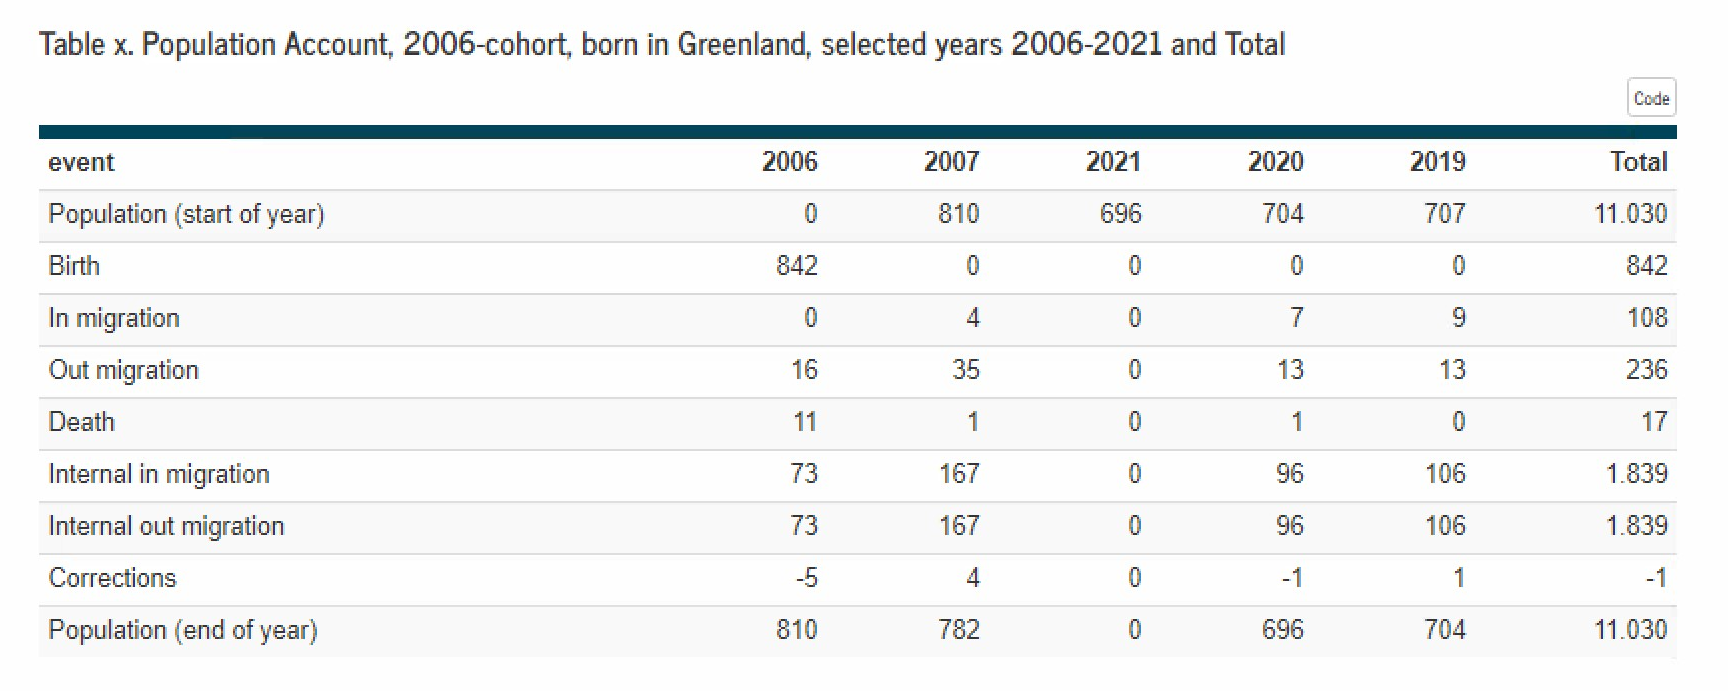
\includegraphics[scale=0.22]{images/PopulationAccountTabX}


\subsection{Population Register from 1973} 

(Statistics Denmark published detailed Population Accounts in BB on paper from 1975-2004)

Statistics on the Greenlandic population are all based on information in our administrative registers with 100 pct national coverage. The base register (CPR) was introduced to Greenland in 1972 and in effect for statistical purposes from 1977. All daily changes to the population’s addresses are recorded, by law, no later than 5 weekdays after occurrence and correctly. This would be a perfect data dream, which in real life, never happens. Even in a ultra small society as the Greenlandic, many hundred persons add changes to the central register annually, so of cause errors are reported, as also events are reported with some delay.

Some events, especially on external migrations are reported more than a year after actual occurrence. Some very few death are also reported very late. According to law, a court can declare ‘presumption of death’ and issue a death certificate for a missing person, no earlier than 10 years after the person has disappeared.

To be current and of use to society statistics can not wait being 100 pct accurate. Instead we aim for the annual statistics to be true and fair. From experience we have chosen to wait 1 calendar month, to allow the register to be updated with delayed reports. We then adjust the population estimate to include events taken place before the report date, January 1st. (or other dates chosen). As long as the number of delayed reported events are approximately the same from one period to the next, the number of events will be approximately equivalent.

But on detailed level (one-year age groups, gender, locality) this will not be true.

Changes in P(opulation) size are described by the vital statistics: B(irths), D(eaths), I(mmigrations) and E(migrations). But because of the delayed reports, a residual calculated c(orrection) post is added to ensure

P(t+1)≡P(t)+B(t)−D(t)+I(t)−E(t)+c(t)
, where t= time

For subnational population calculations internal migration is simply added to this equation.

The correcton post offers important quality information on how well the vital statistics explains changes in population size over time.

As the content is not 100 pct accurate, but true and fair, this serves as a model of the Greenlandic population


\subsection{Statbank Greenland} 
...



\begin{acknowledgement}
  ...
\end{acknowledgement}

%\bibliographystyle{...}
%\bibliography{...}
\end{document}
